\def\year{2021}\relax
%File: formatting-instructions-latex-2021.tex
\documentclass[letterpaper]{article} % DO NOT CHANGE THIS
\usepackage{aaai21}  % DO NOT CHANGE THIS
\usepackage{times}  % DO NOT CHANGE THIS
\usepackage{helvet} % DO NOT CHANGE THIS
\usepackage{courier}  % DO NOT CHANGE THIS
\usepackage[hyphens]{url}  % DO NOT CHANGE THIS
\usepackage{graphicx} % DO NOT CHANGE THIS
\usepackage{array}
\usepackage{multirow}
\usepackage{amsmath}
\usepackage{graphicx}
\usepackage{float}
\usepackage{subfigure}
\usepackage{spconf}
\usepackage{natbib}  % DO NOT CHANGE THIS AND DO NOT ADD ANY OPTIONS TO IT
\usepackage{caption} % DO NOT CHANGE THIS AND DO NOT ADD ANY OPTIONS TO IT

\urlstyle{rm} % DO NOT CHANGE THIS
\def\UrlFont{\rm}  % DO NOT CHANGE THIS
\frenchspacing  % DO NOT CHANGE THIS
\setlength{\pdfpagewidth}{8.5in}  % DO NOT CHANGE THIS
\setlength{\pdfpageheight}{11in}  % DO NOT CHANGE THIS

\providecommand{\tabularnewline}{\\}
%% A simple dot to overcome graphicx limitations
\newcommand{\lyxdot}{.}

\def\x{{\mathbf x}}
\def\L{{\cal L}}

%\nocopyright
%PDF Info Is REQUIRED.
% For /Author, add all authors within the parentheses, separated by commas. No accents or commands.
% For /Title, add Title in Mixed Case. No accents or commands. Retain the parentheses.
\pdfinfo{
  /title (Joint training of classification model and similarity model for
  low-resource text classification in chatbot)
  /Author (no author informmation)
  /TemplateVersion (2021.1)
} 

\setcounter{secnumdepth}{0} %May be changed to 1 or 2 if section numbers are desired.

%%%%%%%%%%%%%%%%%%%%%%%%%%%%%% LyX specific LaTeX commands.
%% Because html converters don't know tabularnewline
\title{     
  %SFC: Few-Shot Text Classification via Similarity Fused with Classification System
  Joint training of classification model and similarity model for low-resource
  text classification in chatbot
}

\begin{document}
  \maketitle

  \begin{abstract}
    Task-specific  chatbot systems have gained many important applications, such
    as  Siri,  Google home, and customer service systems. In these applications,
    one  of  the  core  problems is the intention detection from a user's input.
    Then,  the  intention  with  its  associated  information  is  mapped into a
    predefined dialog logic graph, and the chatbot returns corresponding answer.
    This  is  the  main  difference  from  a  free chatbot system. The intention
    detection,  assuming  only  one  intention  in  a  user's input here, can be
    modeled  as  a  short  text  classification.  In  practice,  the  number  of
    intentions  can  be hundreds of thousands, as opposed to a few number in the
    traditional text classification problem; enough training data is not trivial
    to be filtered out and labeled from tons of raw user logs with miscellaneous
    information, and generally only 10 to 20 samples per intention are available
    in  the  early  stage.  Then,  how  to  train  an  efficient model in such a
    practical  and important application is critical. In this work, we propose a
    novel  model, called similarity model fused with classification Model (SFC),
    which  combines  a  classification  model  and  a similarity model, and also
    borrows  the  power  of  multi-task  training  as well. We conduct extensive
    experiments  on  4  public  and 1 private datasets. The experimental results
    show that our new model outperforms very strong baselines, BERT, RoBERTa and
    ALBERT based pretrained models by 2 percentages in average accuracy.

  \end{abstract}

  \section{Introduction}
  \label{sec:intro}

  Task-specific  conversational  chatbot  \cite{wen2016network}  has been applied
  into  many practical products. For example, it can share the working burden of
  human  customer  service  agents  responsible  for  customers' questions about
  certain  products  or services. Another example is the speech-based control in
  devices  like  intelligent  speakers, such as Siri, Google home, Baidu Xiaodu,
  and smart home equipments. Regardless of whether these conversations belong to
  single-turn or multi-turn, an essential technique underlying the chatbot is to
  identify  the  real  intention  behind  a  user's  question or reply. Then the
  chatbot  is capable of conducting expected actions, text reply or accomplish some
  operations.

  It  is  a  challenging task due to some inherent properties. First,
  a customer's  utterance  within  a conversation is usually quite short. Since it
  does  not  contain  enough  information,  short  text \cite{song2014short} are
  thought  to  be  more  ambiguous  compared to long texts such as paragraphs or
  documents,  posing  a  great challenge \cite{chen2019deep} for classification
  task   \cite{phan2008learning,yan2009dynamic,hua2015short}.   Second,  in  the
  initial  stage  of  building  a  chatbot  , it is often rather hard to collect
  sufficient  labeled  data  to  train  a good model. Because developers have to
  examine tons of real system logs for typical user's utterances, and then label
  them  with expected intentions. Therefore, the key to building a task-specific
  chatbot  with  high  performance  becomes  solving the challenge of short-text
  classification   \cite{sriram2010short}   problem   under   few-shot   setting
  \cite{yu2018diverse}.


  Generally  there  are  two  kinds  of  approaches  to  address  this  problem,
  classification model that directly maps an input into a most likely label, and
  similarity  model  that searches a label whose associated data is most similar to
  an input.


  The   first  one,  \emph{text  classification},  includes  classic  long  text
  classification  and  short  text  classification  in  this  scenario.  Besides
  traditional  machine  learning  models  like  SVM \cite{suykens1999least},  boosting  tree \cite{tu2005probabilistic},  many work
  \cite{wen2016network}  choose  neural  network  such  as  convolutional neural
  networks (CNNs) \cite{kim2014convolutional,zhang2015character,conneau2016very}
  and       long       short       term       memory       networks      (LSTMs)
  \cite{mousa2017contextual,liu2016recurrent}   to   accomplish   the   task  of
  extracting  semantic  feature from limited amount of words. Their common model
  structure  is  adding  a  softmax classifier as the final layer and mapping to
  labels.  Another  two  interesting lines of work, label-word joint models, and
  joint  NER  and  classification  are  discussed  in  the related work section.
  Afterwards,   pre-trained   language   models   on   large  corpus  like  BERT
  \cite{devlin2018bert}  and  RoBERTa \cite{liu2019roberta} has been proven more
  powerful  in  solving  many  NLP  tasks  including  short-text  classification
  \cite{madabushi2020cost}.      Especially      for      few-shot     scenarios
  \cite{yu2018diverse},     pre-trained     model    based    on    transformers
  \cite{vaswani2017attention} tends to do more
  help to reducing the negative effects brought by scarcity of training data.

  The  second  one,  \emph{similarity model} is also called sentence-pair model.
  Its  motivation  originates  from  the idea of Information Retrieval (IR) based
  chatbot   \cite{jafarpour2010filter,   leuski2011npceditor}.   Having   a  Q-A
  (Question-Answer)  pairs dataset and user query Q, the IR based conversational
  system will look up in the Q-A dataset for the pair (Q', A') that best matches
  query  Q  through  semantic  analysis  and  returns  A'  as  the  answer  to Q
  \cite{mnasri2019recent}. In this way, sentence-pair model pre-trained on large
  corpus  of  semantic  similarity  identification task can be applied for being
  used  as  a  tool  to  identify  the class with highest semantic similarity to
  customer's    query.    A    common    model    structure    of    pre-trained sentence-pair model is based on multiple cross-attention
  mechanism  \cite{barkan2020scalable}. Due to
  the   fact   that   many   experiment   results   have   shown   that  RoBERTa
  \cite{liu2019roberta} is an improved version of BERT \cite{devlin2018bert}, and has achieved amazing
  results  on  both  text  classification and sentence-pairs semantic similarity
  tasks, we choose RoBERTa as an important baseline approach in this paper.

  Despite  the  success  of  these two kinds of approaches, they still have some
  limitations   in   task-specific  chatbot  scenario.  As  for  the  \emph{text
  classification  model},  it  is  quite hard to use data augmentation method to
  solve  the  data insufficiency challenge since the it is usually unfeasible to
  get  large amount of domain-specific data when facing a new task. With respect
  to  the  \emph{similarity model}, though we can obtain a large amount of data
  from semantically  duplicate  sentence  pair identification domain for transfer
  learning  \cite{sun2019fine},  it  is  still  quite  hard  to  perform well on
  a new task-specific dataset,  since their objective losses are totally different. 

  The  above limitation motivates us to propose a joint system that is capable of
  taking  advantages  from  both  classification model and similarity model. We
  call  it  SFC,  short  for  similairty model fused with classification Model,
  shown  in  Fig.  \ref{fig:framework}.  To  better train SFC, we further bring in
  multi-task   learning   \cite{caruana1993multitask,collobert2008unified, liu2019multi}.  Our
  basic  idea  came  from  two  stages. In the first stage, we use an auxiliary
  model  to  select top-K most possible labels for a input. This model can be an
  elastic search  \cite{divya2013elasticsearch}  or  a  text classification model
  trained on current task-specific chatbot data. In the second stage, we build a
  classification  model  whose  main modules are similarity models. Then, this
  structure  derives two goals to train towards, the classification loss for our
  application,  and the similarity loss for the main modules. When the two stages
  are  independently  optimized,  we call \emph{two-stage SFC}. We further find,
  the  the  quality  of  output  from  the  first  stage  might  limit the final
  performance  of  system,  since  the  candidate  labels for each user query is
  always  fixed  in  the  whole  multi-task  training  process. This observation
  motivates  us  to  further  improve  the  two-stage SFC into a joint training,
  called  \emph{joint  SFC}. In this way, the sentence pairs associated with the
  top-K  classes  also  become dynamic, and the text classification model in the
  first  stage  will also be further optimized to provide better top-K result by
  the final training loss.


  We summarize our contributions as follow:
  \begin{enumerate}
    \item We propose a novel joint system to makes full utilization of
    the advantages from both text classification model and similarity model.

    \item To  better  train such a system, we bring in multi-task training to obtain
    reasonable performance.

    \item Experiment  results  from 4 public and 1 private short-text classification
    datasets,  show  that  our  proposed  SFC joint system can achieve significant
    and consistent improvements over strong baselines, especially in the low resource settings.
  \end{enumerate}

  \begin{figure*}[t]
    \begin{centering}
      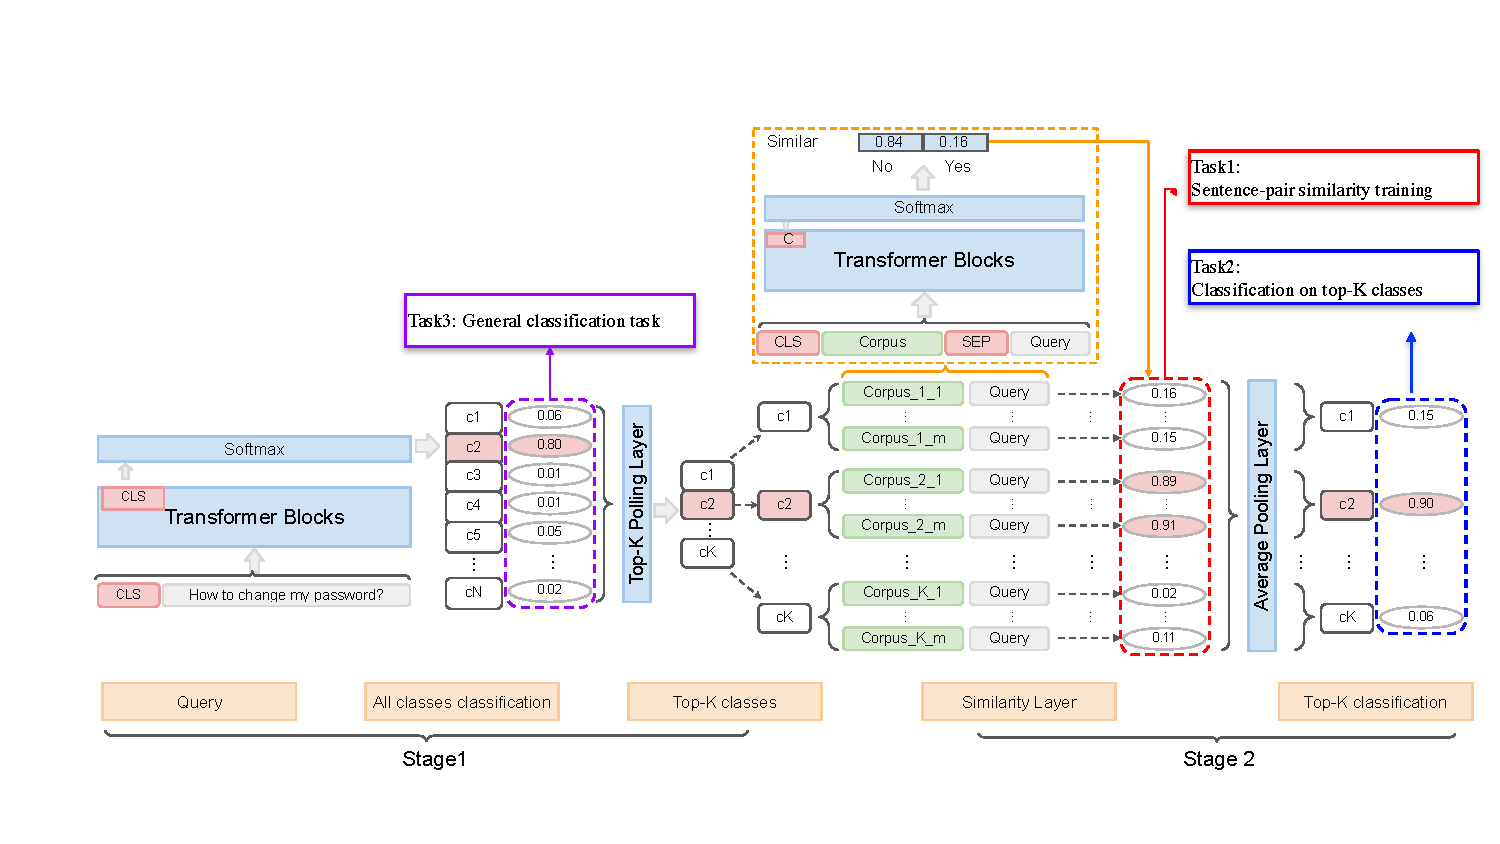
\includegraphics[scale=0.72]{picture/picture4} 
      \par
    \end{centering}
    \caption{
      \textbf{Network Structure of SFC:} two-stage SFC and joint-SFC are sharing
      the  same  network  from  stage  1  and  stage 2, with the only difference
      whether two stages being jointly trained.
    }
    \label{fig:framework}
  \end{figure*}

  \section{Related work}

  Another  common  approach  is  text  classification  neural  network  based on
  label-word     joint     embedding,    such    as    LEAM \cite{wang2018joint},
  MTLE \cite{zhang2017multi}   and   EXAM \cite{du2019explicit}.   This   approach
  involves  label  embedding when constructing the text-sequence representation.
  Take  LEAM  as  an  example,  the  text classification model is implemented by
  jointly    embedding    the    word    and    label   in   the   same   latent
  space \cite{wang2018joint}. Afterwards, the text representation are constructed
  based  on  text-label  compatibility through attention mechanism. In this way,
  additional  sources  of  semantic  information  from class labels can be fully
  leveraged, which is quite helpful especially under few-shot scenario.

  As for \emph{label-word joint
  embedding  approach},  it  poses  noticeable requirements on label information.
  However,  in  our  cases,  since  we have large amount of class labels without
  being well-defined for question answering chatbot, the only thing we can do is
  to  choose  one  of the user utterance as the class label to represent the key
  information  of  the  whole class. In this way, the label will become not only
  prolix  but  also  biased,  which  will  bring  some  negative effect to label
  embedding.  

  Another   line   of  interesting  work  is  the  joint  training  of  sentence
  classification   and  NER  (todo:  reference).  If  both  the  city  and  date
  information  are  recognized,  then  they  are good indicators that this query
  might  be  booking  an  ticket. This work can also be combined in our proposed
  framework.

  \section{Methodology}
  In  this section, we describe our proposed system, similarity model fused with
  classification  model (SFC). We propose two approaches to implement this idea,
  two-stage SFC, and its more unified version joint-SFC.

  \subsection{Two-stage SFC}

  Two-stage   SFC  is  composed  with  two  independent stages  in  charge of
  different  jobs. 

  \subsubsection*{
    Stage 1: classification model for providing top-K candidate class labels
  } 
  We  can  use any auxiliary text classification model or tool,
  such as Term Frequency-Inverse Document Frequency (TF-IDF)retrieval, to
  provide  top-K  most  related  class  labels. These selected class labels will
  later  be  used to sample sentence pairs of both positive samples and negative
  samples  for  stage  2. 

  In  this  work,  we  choose pretrained models to fine tune on our data.
  Due to the excellent performance of RoBERTa in this task, compared to other pretrained
  models, we use RoBERTa as the encoder of classification model in our setting.

  Given   a   data   point   $x_{i}$  with  class  label  $y_{i}$  from  dataset
  $\mathcal{D}$, we take the final hidden state $h_{i}$ of the first token [CLS]
  encoded  by  RoBERTa  as the representation for the whole sequence of $x_{i}$.
  Then  a linear layer is followed to output probabilistic distribution of class
  labels,  $softmax(W^Ch_{i}+b^C)=softmax({\Phi}^C_{i})$,  where $W^C$ and $b^C$
  are  trainable  parameters.  Then, the loss in stage 1 classification model is
  shown in Equ. \ref{eq:classification_loss},


  \begin{equation}
    \begin{aligned}
      \mathcal{L}^{C}&=\frac{1}{N}\sum_{i=1}^{N}-log(\frac{exp(\varPhi_{i,y_{i}}^C)}{\sum_{j=1}^{C}exp(\varPhi_{i,j}^C)}) \\
      \label{eq:classification_loss}
    \end{aligned}
  \end{equation}

  \subsubsection*{
    Stage 2: sentence-pair similarity model based classification with multi-task
    learning
  }
  We  continue choosing RoBERTa as the main module in this stage that identifies
  the class label with strongest semantic similarity to the user input sentence.

  Suppose  we have a training dataset $\mathcal{D}=\{x_{i},y_{i}\}_{i=1}^{N}$ of
  $N$  data  points,  in  which $x_{i}$ is the user input query and $y_{i}$ is a
  single  class label from a class label set of $C$ classes in total. We 
  generate            a sentence            pair            dataset
  $\mathcal{D'}=\{[(x,x')_{j},l_{j}]\}_{j=1}^{M}$ from $\mathcal{D}$,   where   $(x,   x')_{j}$  is
  a pair of two history queries \footnote{For simplicity, we use query
  to denote a user's question or a response.}, and $l_{j}\in\{0, 1\}$ denotes the
  similarity label that the ones from the same class label are considered
  similar. The size of $\mathcal{D'}$  would be up to $O(N^2)$ if no any
  sampling strategy is used.  This is quite time-consuming  for the  training
  in stage 2 because $N$ can be several hundreds or thousands even under 
  few shot setting in task-specific chatbot scenario. 

  Therefore,  we  adopt  the idea of adversarial negative sampling strategy from
  the  work  \cite{bamler2020extreme}.  The  key  idea is to train with negative
  samples  that  are hard to be distinguished from positive samples. Now suppose
  we  have  a  user  input query $x_{i}$ and top-K most related class labels set
  $\mathcal{C'}=\{c'_{1},  \dots,  c'_{K}\}$ provided by auxiliary model or tool
  in  stage  1, where $K$ is a hyperparameter to control candidate class number,
  we  apply  the  adversarial  negative sampling strategy into our sentence pair
  sampling process by the following two steps:

  The  first step is \emph{positive sentence pair sampling}. During the training
  process,  we  first make sure the ground truth class label $y_{i}$ for $x_{i}$
  is  within  the  candidate  class  label  set  $\mathcal{C'}$. If $y_{i}\notin
  \mathcal{C'}$,  we  manually  add  $y_{i}$  into  $\mathcal{C'}$  by replacing
  $c'_{K}$  with  $y_{i}$, since $c'_{K}$ is the least promising candidate label
  according  to  the  auxiliary  model  in stage 1. Afterwards, we will randomly
  sample  $P$ sentences $\{x'_{1}, \dots, x'_{P}\}$ with the same class label as
  $y_{i}$  from  dataset  $\mathcal{D}$  to  form the set of sentence pairs with
  positive  label  $\mathcal{P'}_{i}=\{[(x_{i},  x'_{1}),  1],  \dots,  [(x_{i},
  x'_{P}),  1]\}$,  where $P$ is also a hyperparameter set to control the number
  of sentences we should sample from each class.

\begin{table*}
    \begin{centering}
      \scalebox{0.9}{
        \begin{tabular}{|c|c|c|c|c|c|}
          \hline 
          \textbf{Dataset} & \textbf{Domain} & \textbf{\#Class} &
          \textbf{\#Training Samples} & \textbf{\#Samples/Class} & \textbf{Experimental Settings}\tabularnewline
          \hline 
          ITG & FAQ chatbot & 228 & 3938 & 17 & 3-fold\tabularnewline
          \hline 
          Amazon-670k & Product review & 250 & 1942 & 8 & 3-fold\tabularnewline
          \hline 
          HWU64 & intention detection & 64 & [320, 640, 960, 1280, 1920, 3200] & [5, 10, 15, 20, 30, 50] & data sampling\tabularnewline
          \hline 
          CLINC150 & intention detection & 150 & [750, 1500, 2250, 3000, 4500, 7500] & [5, 10, 15, 20, 30, 50] & data sampling\tabularnewline
          \hline 
          BANKING77 & intention detection & 77 & [385, 770, 1155, 1540, 2310, 3850] & [5, 10, 15, 20, 30, 50] & data sampling\tabularnewline
          \hline 
        \end{tabular}
      }
      \par
    \end{centering}
    \caption{Statistics for all datasets and few shot settings\footnote{All
    settings of four public datasets would be released to github soon}.}

    \label{tbe:dataset statistic}
  \end{table*}


  The  second  step  is  \emph{negative sentence pair sampling}: As for negative
  sentence  pairs,  we will also randomly sample $P$ sentences for each class in
  the negative candidate class label set $\mathcal{C'}\backslash \{y_{i}\}$. The
  class  labels  in  $\mathcal{C'}\backslash  \{y_{i}\}$  are  the  set  of most
  confusing  class  labels comparing to the ground truth ${y_{i}}$, so we assume
  that  the  sentence  pairs  with  negative  label  grouped by user input query
  $x_{i}$  and sentences with class labels in $\mathcal{C'}\backslash \{y_{i}\}$
  are  strong  adversarial  negative  samples for sentence-pair similarity model
  that  can  help  enhance  the training speed and performance. According to the
  same  method  as  positive  sentence  pair  sampling, we can obtain the set of
  sentence  pairs  with  negative label as $\mathcal{N'}_{i}=\{[(x_{i}, x'_{1}),
  0], ..., [(x_{i}, x'_{P\cdot (K-1)}), 0]\}$

  In  this way, we generate the sentence pair dataset $\mathcal{D'}$ for stage 2
  based  on  the  top-K  class  label  set $\mathcal{C'}$ provided by stage 1 as
  $\mathcal{D'}=\{\mathcal{P'}_{i}\cup  \mathcal{N'}_{i}\}_{i=1}^{N}$,  in which
  we have $M=N\cdot K\cdot P$ data points of sentence pairs in total.

  Before starting to fine-tune our sentence-pair model on task-specific dataset,
  we  first  fine-tune  RoBERTa  on  Quora  dataset  \cite{iyer2017first}, which
  contains  404,290  potential  duplicate question pairs, for transfer learning.
  This  is  also  the  merit of similarity based model, as labeled task-specific
  classification  data  is  hard  to  acquire,  yet  general sentence pairs with
  similar semantics can be much easier to acquire.

  \subsubsection*{Multi-task based training}
  We   continue  to  do  multi-task  training  on  sentence-pair  dataset
  $\mathcal{D'}$ sampled from the top-K candidate class labels provided by stage
  1. In stage 2, we have two tasks tuning our system.

  The first task is \emph{regular sentence-pair similarity task}.
  For  sentence  pair semantic similarity task, given a data point $(x, x')_{i}$
  with       similarity       label       $l_{i}$       from       data      set
  $\mathcal{D'}=\{[(x,x')_{i},l_{i}]\}_{i=1}^{M}$,   Roberta   takes  the  final
  hidden  state  $h_{i}$  of the first token [CLS] as the representation for the
  sequence of packed sentence pair $(x, x')_{i}$. Let's suppose we have a linear
  layer  as  ${\Phi}^S_{i}=W^Sh_{i}+b^S$,  where  $W^S$  and $b^S$ are trainable
  parameters,  and  the probability score for $(x, x')_{i}$ can be calculated as
  $p^S_{i}=softmax({\Phi}^S_{i})$.

  Due  to  the  fact that sentence pairs within the same class is much fewer than
  that from  different  classes,  the  dataset  $\mathcal{D'}$  is
  quite imbalanced.  Therefore, we will accommodate a weight variable $w^S = [K-1, 1]$
  to  the  loss  to eliminate the bias brought by data imbalance, shown in Equ.
  \ref{eq:similarity_loss}.

  \begin{equation}
    \begin{aligned}
      \mathcal{L}^{S}&=\frac{1}{M}\sum_{i=1}^{M}-w^S_{l_i}\cdot log(\frac{exp(\varPhi_{i,l_{i}}^S)}{\sum_{j=0}^{1}exp(\varPhi_{i,j}^S)}) \\
      \label{eq:similarity_loss}
    \end{aligned}
  \end{equation}

  The  second  task  is  \emph{classification  on  top-K classes}. As minimizing
  similarity  loss  is  not  our  final goal in the intention classification, we
  bring  back  classification  loss again. In this task, the network is based on
  sentence  pair  similarity  modules.  The  only  difference  is  that we add a
  task-specific  average  pooling  layer,  shown  in Fig. \ref{fig:framework} to
  accomplish the classification task based on sentence-pair model.

  We  already  know  that the size of ${\Phi}^S$ in task 1 is $M\times 2=(N\cdot
  K\cdot  P)\times  2$, where $N$ is the total number of data points in original
  training  data $\mathcal{D}$, $K$ is a hyperparameter that controls the number
  of   candidate   class  labels  provided  by  stage  1,  and  $P$  is  also  a
  hyperparameter that controls the number of sentences we should randomly sample
  from each candidate class labels. Now, for the average pooling layer, we first
  reshape  ${\Phi}^S$  into  the  size  of $N\times K\times P\times 2$, and then
  split  it  into  ${\Phi}^{K,pos}$  and ${\Phi}^{K,neg}$, and both of them will
  have  the  size  of  $N\times  K\times  P$.  In this way, ${\Phi}^{K,pos}$ can
  represent  the  level  of  similarity  for each sentence pair, and in the mean
  time,  ${\Phi}^{K,neg}$  can  represent  the  level  of dissimilarity for each
  sentence  pair. Then, we can do average pooling for each candidate class among
  the  top-K  classes  as  shown  in  Equ.  \ref{eq:average  pooling}.

  \begin{align}
    {\xi}_{i,j}^{K,pos} = \sum_{p=1}^{P}{\varPhi}_{i,j,p}^{K,pos} \ \ \ \ \ \ \ 
    {\xi}_{i,j}^{K,neg} = \sum_{p=1}^{P}{\varPhi}_{i,j,p}^{K,neg}
    \label{eq:average pooling}
  \end{align}

  With  the  average pooling result ${\xi}^{K,pos}$ and ${\xi}^{K,neg}$, we also
  generate   a   top-K   class   label   $l^{K}_i\in   [1,\dots,K]$   for   each
  ${\xi}^{K,pos}_{i}$ and ${\xi}^{K,neg}_{i}$. The loss for top-K classification
  task is shown in Equ. \ref{eq:top-k_classification_loss}. In Equ. \ref{eq: pos
  top-k   loss}   and   Equ.   \ref{eq:   neg   top-k   loss},  the  first  term
  $\xi_{i,l^{K}_{i}}^{K,pos}$  and  $\xi_{i,l^{K}_{i}}^{K,neg}$  encourage  high
  level  of  similarity  and  low  level  of dissimilarity for prediction of the
  correct label $l^{K}_i$ within the top-K candidate classes.

  \begin{align}
    \mathcal{L}^{K} = \frac{1}{N}\sum_{i=1}^{N}(\mathcal{L}^{K,pos}_{i} - \mathcal{L}^{K,neg}_{i})
    \label{eq:top-k_classification_loss}
  \end{align}
  where

  \begin{equation}
    \begin{aligned}
      \mathcal{L}^{K,pos}_{i} &= -log(\frac{exp(\xi_{i,l^{K}_{i}}^{K,pos})}{\sum_{j=1}^{K}exp(\xi_{i,j}^{K,pos})})
      \label{eq: pos top-k loss}
    \end{aligned}
  \end{equation}

  \begin{equation}
    \begin{aligned}
      \mathcal{L}^{K,neg}_{i} &= -log(\frac{exp(\xi_{i,l^{K}_{i}}^{K,neg})}{\sum_{j=1}^{K}exp(\xi_{i,j}^{K,neg})}) \\
      \label{eq: neg top-k loss}
    \end{aligned}
  \end{equation}

  Finally,  the  overall  loss  function for multi-task learning in stage 2 is
  shown in Equ. \ref{eq:two-stage_SFC_loss}. The training objective of stage 2 is
  to  minimize  the  weighted  sum  of task-specific losses. Here $\alpha_S$ and
  $\alpha_K$  are  weights  of  task  1  and  task  2  respectively.

  \begin{align}
    \mathcal{L} = \alpha_S \mathcal{L}^S + \alpha_K \mathcal{L}^K
    \label{eq:two-stage_SFC_loss}
  \end{align}

  
  \begin{table*}
    \begin{centering}
      \scalebox{0.55}{
        \begin{tabular}{|c|cccccc|cccccc|cccccc|c|c|}
          \hline 
          \multicolumn{1}{|c|}{\multirow{2}*{\textbf{Models}} }& \multicolumn{6}{c|}{\textbf{CLINC150}}& \multicolumn{6}{c|}{\textbf{BANKING77}}& \multicolumn{6}{c|}{\textbf{HWU64}}& \ \ \ \textbf{ITG} \ \ \ & \textbf{Amazon-670k}\tabularnewline
          \cline{2-21}
          \multicolumn{1}{|c|}{} & $\textbf{5}$ & $\textbf{10}$ & $\textbf{15}$
          & $\textbf{20}$ & $\textbf{30}$ & $\textbf{50}$ & $\textbf{5}$ &
          $\textbf{10}$ & $\textbf{15}$ & $\textbf{20}$ & $\textbf{30}$ &
          $\textbf{50}$ & $\textbf{5}$ & $\textbf{10}$ & $\textbf{15}$ &
          $\textbf{20}$ & $\textbf{30}$ & $\textbf{50}$ & \textbf{3-fold} &
          \textbf{3-fold}\tabularnewline
          \hline
          TextCNN & \multirow{2}*{$0.5318$} & \multirow{2}*{$0.6963$} & \multirow{2}*{$0.7609$} & \multirow{2}*{$0.8142$} & \multirow{2}*{$0.8526$} & \multirow{2}*{$0.8867$} & \multirow{2}*{$0.4408$} & \multirow{2}*{$0.6436$} & \multirow{2}*{$0.7366$} & \multirow{2}*{$0.7918$} & \multirow{2}*{$0.8228$} & \multirow{2}*{$0.8619$} & \multirow{2}*{$0.3112$} & \multirow{2}*{$0.4007$} & \multirow{2}*{$0.4823$} & \multirow{2}*{$0.5272$} & \multirow{2}*{$0.5782$} & \multirow{2}*{$0.6262$} & \multirow{2}*{$0.6624$} & \multirow{2}*{$0.4401$}\tabularnewline
          (classification) & & & & & & & & & & & & & & & & & & & &\tabularnewline
          LEAM & \multirow{2}*{$0.7514$} & \multirow{2}*{$0.8203$} & \multirow{2}*{$0.8612$} & \multirow{2}*{$0.8802$} & \multirow{2}*{$0.9010$} & \multirow{2}*{$0.9180$} & \multirow{2}*{$0.5422$} & \multirow{2}*{$0.7812$} & \multirow{2}*{$0.8129$} & \multirow{2}*{$0.8280$} & \multirow{2}*{$0.8610$} & \multirow{2}*{$0.8727$} & \multirow{2}*{$0.4545$} & \multirow{2}*{$0.5554$} & \multirow{2}*{$0.5936$} & \multirow{2}*{$0.6599$} & \multirow{2}*{$0.6855$} & \multirow{2}*{$0.7046$} & \multirow{2}*{$0.7086$} & \multirow{2}*{$0.6091$}\tabularnewline
          (classification) & & & & & & & & & & & & & & & & & & & &\tabularnewline
          \hline
          BERT-large & \multirow{2}*{$0.8080$} & \multirow{2}*{$0.8904$} & \multirow{2}*{$0.9265$} & \multirow{2}*{$0.9334$} & \multirow{2}*{$0.9497$} & \multirow{2}*{$0.9595$} & \multirow{2}*{$0.5780$} & \multirow{2}*{$0.8004$} & \multirow{2}*{$0.8518$} & \multirow{2}*{$0.8827$} & \multirow{2}*{$0.8858$} & \multirow{2}*{$0.8982$} & \multirow{2}*{$0.4711$} & \multirow{2}*{$0.5963$} & \multirow{2}*{$0.6342$} & \multirow{2}*{$0.7010$} & \multirow{2}*{$0.7117$} & \multirow{2}*{$0.7424$} & \multirow{2}*{$0.7485$} & \multirow{2}*{$0.6658$}\tabularnewline
          (classification) & & & & & & & & & & & & & & & & & & & &\tabularnewline
          ALBERT-xxlarge & \multirow{2}*{$0.8497$} & \multirow{2}*{$0.9008$} & \multirow{2}*{$0.9296$} & \multirow{2}*{$0.9297$} & \multirow{2}*{$0.9466$} & \multirow{2}*{$0.9578$} & \multirow{2}*{$0.5549$} & \multirow{2}*{$0.7981$} & \multirow{2}*{$0.8231$} & \multirow{2}*{$0.8530$} & \multirow{2}*{$0.8571$} & \multirow{2}*{$0.9096$} & \multirow{2}*{$0.4879$} & \multirow{2}*{$0.6116$} & \multirow{2}*{$0.6135$} & \multirow{2}*{$0.6996$} & \multirow{2}*{$0.7094$} & \multirow{2}*{$0.7376$} & \multirow{2}*{$0.7253$} & \multirow{2}*{$0.6893$}\tabularnewline
          (classification) & & & & & & & & & & & & & & & & & & & &\tabularnewline
          RoBERTa-base & \multirow{2}*{$0.8732$} & \multirow{2}*{$0.9254$} & \multirow{2}*{$0.9363$} & \multirow{2}*{$0.9482$} & \multirow{2}*{$0.9558$} & \multirow{2}*{$0.9637$} & \multirow{2}*{$0.7305$} & \multirow{2}*{$0.8654$} & \multirow{2}*{$0.8808$} & \multirow{2}*{$0.9080$} & \multirow{2}*{$0.9061$} & \multirow{2}*{$0.9293$} & \multirow{2}*{$0.5831$} & \multirow{2}*{$0.6790$} & \multirow{2}*{$0.7064$} & \multirow{2}*{$0.7100$} & \multirow{2}*{$0.7320$} & \multirow{2}*{$0.7472$} & \multirow{2}*{$0.7734$} & \multirow{2}*{$0.6708$}\tabularnewline
          (classification) & & & & & & & & & & & & & & & & & & & &\tabularnewline
          \hline
          RoBERTa-large & \multirow{2}*{$\textbf{0.8974}$} &
          \multirow{2}*{$\textbf{0.9372}$} & \multirow{2}*{$\textbf{0.9508}$} &
          \multirow{2}*{$\textbf{0.9584}$} & \multirow{2}*{$\textbf{0.9621}$} & 
          \multirow{2}*{$\textbf{0.9733}$} & \multirow{2}*{$\textbf{0.7690}$} & 
          \multirow{2}*{$\textbf{0.8728}$} & \multirow{2}*{$\textbf{0.8966}$} & 
          \multirow{2}*{$\textbf{0.9099}$} & \multirow{2}*{$\textbf{0.9227}$} & 
          \multirow{2}*{$\textbf{0.9313}$} & \multirow{2}*{$\textbf{0.6044}$} & 
          \multirow{2}*{$\textbf{0.7002}$} & \multirow{2}*{$\textbf{0.7129}$} & 
          \multirow{2}*{$\textbf{0.7436}$} & \multirow{2}*{$\textbf{0.7493}$} & 
          \multirow{2}*{$\textbf{0.7678}$} & \multirow{2}*{$\textbf{0.7990}$} & 
          \multirow{2}*{$\textbf{0.7156}$}\tabularnewline
          (classification) & & & & & & & & & & & & & & & & & & & &\tabularnewline
          RoBERTa-large & \multirow{2}*{$0.8266$} & \multirow{2}*{$0.8861$} & \multirow{2}*{$0.9023$} & \multirow{2}*{$0.9084$} & \multirow{2}*{$0.9090$} & \multirow{2}*{$0.9407$} & \multirow{2}*{$0.757$} & \multirow{2}*{$0.8476$} & \multirow{2}*{$0.8614$} & \multirow{2}*{$0.8743$} & \multirow{2}*{$0.8749$} & \multirow{2}*{$0.8980$} & \multirow{2}*{$0.5425$} & \multirow{2}*{$0.6164$} & \multirow{2}*{$0.6503$} & \multirow{2}*{$0.6729$} & \multirow{2}*{$0.6947$} & \multirow{2}*{$0.7231$} & \multirow{2}*{$0.7418$} & \multirow{2}*{$0.6362$}\tabularnewline
          (similarity) & & & & & & & & & & & & & & & & & & & &\tabularnewline
          \hline
          2-stage SFC & \multirow{2}*{$0.8979$} & \multirow{2}*{$0.9457$} & \multirow{2}*{$0.9517$} & \multirow{2}*{$0.9591$} & \multirow{2}*{$0.9610$} & \multirow{2}*{$0.9664$} & \multirow{2}*{$0.7975$} & \multirow{2}*{$0.8818$} & \multirow{2}*{$0.8962$} & \multirow{2}*{$0.9109$} & \multirow{2}*{$0.9187$} & \multirow{2}*{$0.9198$} & \multirow{2}*{$0.6477$} & \multirow{2}*{$0.7055$} & \multirow{2}*{$0.7200$} & \multirow{2}*{$0.7232$} & \multirow{2}*{$0.7484$} & \multirow{2}*{$0.7653$} & \multirow{2}*{$0.7972$} & \multirow{2}*{$0.7189$}\tabularnewline
          (task1) & & & & & & & & & & & & & & & & & & & &\tabularnewline
          2-stage SFC & \multirow{2}*{$0.9162$} & \multirow{2}*{$0.9424$} & \multirow{2}*{$0.9530$} & \multirow{2}*{$0.9617$} & \multirow{2}*{$0.9633$} & \multirow{2}*{$0.9690$} & \multirow{2}*{$0.7997$} & \multirow{2}*{$0.8823$} & \multirow{2}*{$0.8945$} & \multirow{2}*{$0.9123$} & \multirow{2}*{$0.9236$} & \multirow{2}*{$0.9317$} & \multirow{2}*{$0.6498$} & \multirow{2}*{$0.6980$} & \multirow{2}*{$0.7202$} & \multirow{2}*{$0.7358$} & \multirow{2}*{$0.7498$} & \multirow{2}*{$0.7657$} & \multirow{2}*{$0.8020$} & \multirow{2}*{$0.7311$}\tabularnewline
          (task2) & & & & & & & & & & & & & & & & & & & &\tabularnewline
          2-stage SFC & \multirow{2}*{$0.9167$} & \multirow{2}*{$0.9456$} & \multirow{2}*{$0.9571$} & \multirow{2}*{$0.9638$} & \multirow{2}*{$0.9658$} & \multirow{2}*{$0.9753$} & \multirow{2}*{$0.8135$} & \multirow{2}*{$0.8854$} & \multirow{2}*{$0.8931$} & \multirow{2}*{$0.9192$} & \multirow{2}*{$0.9257$} & \multirow{2}*{$0.9339$} & \multirow{2}*{$0.6525$} & \multirow{2}*{$0.7092$} & \multirow{2}*{$0.7168$} & \multirow{2}*{$0.7476$} & \multirow{2}*{$0.7519$} & \multirow{2}*{$0.7696$} & \multirow{2}*{$\textbf{0.8124}$} & \multirow{2}*{$0.7364$}\tabularnewline
          (task1 + task2) & & & & & & & & & & & & & & & & & & & &\tabularnewline
          \hline
          \multirow{2}*{Joint SFC} & \multirow{2}*{$\textbf{0.9231}$} & \multirow{2}*{$\textbf{0.9560}$} & \multirow{2}*{$\textbf{0.9644}$} & \multirow{2}*{$\textbf{0.9669}$} & \multirow{2}*{$\textbf{0.9712}$} & \multirow{2}*{$\textbf{0.9821}$} & \multirow{2}*{$\textbf{0.8270}$} & \multirow{2}*{$\textbf{0.9069}$} & \multirow{2}*{$\textbf{0.9103}$} & \multirow{2}*{$\textbf{0.9209}$} & \multirow{2}*{$\textbf{0.9323}$} & \multirow{2}*{$\textbf{0.9463}$} & \multirow{2}*{$\textbf{0.6697}$} & \multirow{2}*{$\textbf{0.7211}$} & \multirow{2}*{$\textbf{0.7254}$} & \multirow{2}*{$\textbf{0.7497}$} & \multirow{2}*{$\textbf{0.7593}$} & \multirow{2}*{$\textbf{0.7772}$} & \multirow{2}*{$0.8114$} & \multirow{2}*{$\textbf{0.7445}$}\tabularnewline
          & & & & & & & & & & & & & & & & & & & &\tabularnewline
          \hline
        \end{tabular}
      }
      \par
    \end{centering}
    \caption{
      F1 scores  on  five  task-specific  datasets text classification in chatbot
      under low resource. For ITG, we keep the full dataset. For Amazon-670k, we
      randomly  sampled  250  classes  with  training sample numbers within 5-15
      samples  per  class.  For  CLINC150,  BANKING77,  HWU64, we set up various
      few-shot  settings  (5/10/15/20/30/50 samples per class) while keeping the
      test  set to be fixed. The highest scores among all the baseline models and SFC variants for each data setting are both marked
      in bold.
    }
    \label{tbe:table2}
  \end{table*}



  \subsection{Joint SFC}
  In  two-stage  SFC,  Stage  1  and  stage 2 are separate that there is no deep
  interaction  with each other during training. In this case, the performance of
  stage  1  may  limit  the potential of stage 2; meanwhile, stage 2 also cannot
  give  training feedback back to stage 1 for fine-tuning. Therefore, to further
  improve  the  overall performance of SFC, we proposed a joint model structure,
  shown in Fig. \ref{fig:framework}.

  In  joint  SFC,  classification  model is being placed in lower layer level to
  dynamically  provide  top-K  candidate  class  labels  for  the  sentence-pair
  similarity  model  placed in higher layer level through a top-K pooling layer.
  In  this way, classification model and similarity model can be merged into one
  single  joint-model  for  multi-task training with sentence pairs sampled from
  varying  candidate  class  labels,  thus  avoiding the limitation brought by 2
  separate stage structure.

  There  are 3 tasks in total during the training process of joint SFC, shown in
  Fig. \ref{fig:framework}, and the overall loss is also the weighted sum of all
  the   task-specific  losses,  shown  in  Equ.  \ref{eq:joint_SFC_loss}.  Here,
  $\alpha_S$,  $\alpha_K$  and  $\alpha_C$  represent  the  weights  for  task 1
  sentence-pair  similarity  in  Equ.  \ref{eq:similarity_loss},  task  2  top-K
  classification  in Equ. \ref{eq:top-k_classification_loss}, and task 3 general
  single       sentence       classification      respectively      in      Equ.
  \ref{eq:classification_loss}.

  \begin{align}
    \mathcal{L} = \alpha_S \mathcal{L}^S + \alpha_K \mathcal{L}^K + \alpha_C \mathcal{L}^C
    \label{eq:joint_SFC_loss}
  \end{align}

  \section{Experiments}
  \label{sec:exp}

  \subsection{Datasets}
  Our experiments aim to study the short text classification in the low-resource
  environment  popular  in  the  task-specific conversational chatbot application.
  Hence we choose and configure set datasets to serve this study. Different from
  the  datasets from other short text classification research, such as semantics
  classification  with  very  limited  semantics labels and relatively longer
  input,   the   datasets  adopted  in  our  experiments  are  typically  having
  comparatively  large  number  of  class labels, ranging from several dozens to
  hundreds,  and  each  class  label  is  associated  with  a handful of labeled
  queries with each  query  being usually  one  sentence. Table \ref{tbe:dataset
  statistic} displays their statistics.

  \begin{enumerate}
    \item \emph{ITG},  is  a proprietory FAQ dataset from real-world
    chatbot  project,  which is composed of question and answer pairs about online
    English teaching. It contains 3,938 sample questions for 228 class labels, and
    each class label corresponds to a unique answer.

    \item \emph{Amazon-670K}, is a customer product review dataset for
    text  classification  task  from  the  extreme  classification repository. The
    complete  dataset  contains 670,091 class labels, 285,176 training samples and
    150,875   testing   samples   \cite{bhatia2016extreme}.  As  each  sample  may
    correspond  to  multiple  class labels, we keep only the first one. We further
    filter  out the class labels that each one is associated with 5 to 15 samples,
    or  reviews,  to  mimic  the  chatbot scenario. From them, we sample 250 class
    labels as well as their samples to form a subset with 1,942 + 716 samples.

    \item \emph{HWU64}, is a intention detection dataset designed for
    home  robot  scenario \cite{liu2019benchmarking}. It aims at the specific task
    of  capturing  the  intention  for  different  user requests to home robot and
    finding  the corresponding answer. The raw dataset contains 25,716 data points
    for 64 class labels through crowdsourcing.

    \item \emph{CLINC150},  is  a dataset designed for task-oriented
    systems  with  23,700 queries that are short and unstructured for 150 intents,
    in    the    same   style   made   by   real   users   through   crowdsourcing
    \cite{larson2019evaluation}.

    \item \emph{BANKING77}, is a intention detection dataset for bank
    customer  services.  The  raw dataset contains 13,084 data points for 77 class
    labels \cite{casanueva2020efficient}.
  \end{enumerate}

  Regarding  the first two datasets, we conduct 3-fold cross validation experiments
  that   70   percent   as  training,  15  percent  as  validation  and  testing
  respectively,  and  report  the  averaged  testing results. Regarding the last
  three datasets, we conduct experiments using a sampling method similar to that
  in   \cite{casanueva2020efficient}   yet  in  a  more  sophisticated  few-shot
  settings.  We  fix  a  test  data for each one, and examine their performances
  using  5,  10,  15,  20,  30,  and 50 samples per class label respectively for
  training.  This  is important, as in practice, a task-specific chatbot usually
  starts  with  merely  a  handful of labeled data available in the early stage.
  Besides,  in  the  active  learning framework, building an effective auxiliary
  system  with limited resource is also quite important to help developers label
  data more efficiently.

  \subsection{Baselines}
  We choose three kinds of system to construct our baselines.

  \begin{enumerate}
    \item \emph{Pretrained model based classification system}, which consists of
    BERT \cite{devlin2018bert},  RoBERTa \cite{liu2019roberta},  and  ALBERT  \cite{lan2019albert}  based.  These pretrained
    models  are  practically  proven  to  achieve  outstanding  performances  in
    classification task and other NLP tasks.

    \item   \emph{Non-pretrained   model  based  classification  system},  which
    consists  of  a typical CNN based TextCNN \cite{kim2014convolutional}, and a
    label-embedding based LEAM \cite{wang2018joint}. Regarding TextCNN, the
    model is based on output from RoBERTa tokenization, and the kernels are set
    as 1, 2, 3, 4, 5. Regarding LEAM, a literal class label is required, which
    is available only in HWU64, CLINC150, BANKING77. Thus, for other two
    datasets, we have to use its class number instead.  Empirically,
    a  non-pretrained  model  based  system  are  not  performing  as  well as a
    pretrained  models  based,  if  both is applicable in some task. Our listing
    these  non-pretrained model based systems here is to provide a comprehensive
    performance comparison on our datasets.

    \item   \emph{Pre-trained   model   based   similarity   model}.  We  choose
    RoBERTa-large  as  our  fundamental  module as our SFC systems are based on
    RoBERTa  too, and RoBERTa is empirically more effective than other pretrained
    models  in  the  short  text  classification  task  in  our  experiments. In
    inference,  we  use  an  elastic search to find a set of potential candidate
    labels for the similarity model, to guarantee a reasonable running time.
  \end{enumerate}

  Our SFC systems include two-stage SFC with ablation, trained with two tasks
  separately and both, and joint SFC with all three tasks.

  \subsection{Implementation Details}
  For  our  SFC  systems,  we  use RoBERTa-large as the pretrained model for both
  classification  task  and  sentence-pair similarity task. We fine-tune
  our  SFC  system  on  our datasets with max sequence length of 128,
  learning  rate  of 1.5e-5 for RoBERTa-large pretrained model and learning rate
  of  5e-4  for  task-specific  layer  with polynomial decay and Adam optimizer.
  Besides,  we  set  the  max number of the epoch to 100 and save the best model on
  validation  set based on testing result in weighted F1 score (todo: reference). 
  We report the F1 score as the main evaluation measure for all experiments.

  In two-stage SFC, in equ. \ref{eq:two-stage_SFC_loss} the weights of two tasks
  are  set  as  $\alpha_S=0.125$ and $\alpha_K=0.875$ in our setting. The reason
  for  giving  task  2 relatively more weights is that according to the ablation
  experiments  we  did  in Section \ref{sec:exp}, task 2 contributes more to the
  overall  performance.  In  joint  SFC,  in  equ.  \ref{eq:joint_SFC_loss}, the
  weights  of  three  tasks  are  set  as  $\alpha_S=0.25$,  $\alpha_K=0.25$ and
  $\alpha_C=0.5$  in  our setting. Overall, the task weights are less sensitive
  in Joint SFC than in two-stage SFC.

  For  the  experiments  in  Table  \ref{tbe:table2},  we  empirically  set  the
  hyperparameter  to  be  $K=5$  and  $P=10$  for  all  SFC  variants.  In Table
  \ref{tbe:table3},  we  conduct extensive experiments to see the performance of
  SFC system under various hyperparameter settings.

  \subsection{Result Analysis}
  All results in F1 score (todo: reference) on the five datasets with different models and configurations are
  showed in Table  \ref{tbe:table2}.

  The performance of each model is measured in F1 score on the fixed
  test  set  for  each  dataset.  
  Overall,  two-stage  SFC systems in multi-task training deliver  moderate 
  improvements  over  corresponding baselines, and joint SFC deliver more
  significant and consistent improvements over the best baseline, RoBERTa based
  classification. In following content, we dive into more details.

  \subsubsection*{Are multi-task and joint training working?} 
  First, we compare the four  SFC  variants to analyze the improvement
  brought  by  multi-task  and  joint-model  structure. 

  \begin{table}
    \begin{centering}
      \begin{tabular}{|c|c|c|c|c|}
        \hline
        F1 score & Two-stage SFC & Joint SFC & Gap & \tabularnewline
        \hline
        top-1 accuracy  & \textbf{81.50} & 81.07 & -0.47 & \tabularnewline
        top-5 accuracy & 94.01 & \textbf{94.30} & +0.29 & \tabularnewline
        \hline
      \end{tabular}
      \par
    \end{centering}
    \caption{The average classification accuracy in stage 1 on all five dataset.}
    \label{tbe:top1_5_accuracy}
  \end{table}

  Comparing with training two-stage SFC with multi-task, training with only task
  1,  namely the sentence pair similarity model, degrades by 0.8 percent
  point  on average, and training with only task 2, namely the top-K based
  classification  task,  degrades  by  0.45  percent  point  on  average.  These
  degradation  indicates  multi-task training in two-stage SFC is helpful for the
  system  performance.  Besides, task 2 plays a relatively more important role in
  multi-task learning, and this aligns with their optimal weight settings.

  Joint SFC consistently outperforms two-stage SFC with multi-task training  
  on 5 diverse datasets by 0.95 percents  on  average. 
  This observation supports the idea that the joint model
  structure  can  alleviate  the  limitation  brought by the lack of interaction
  between  two  stages.  In  following analysis, we will focus on the comparison
  between joint SFC and the other baseline models.

  \subsubsection*{Is  the  fusion of a classification model and a similarity model
  helpful?}  We  compare  the performance of joint SFC with classification based
  and similarity based baselines.

  \begin{table*}
    \begin{centering}

      \begin{tabular}{|c|c|c|c|c|c|c|}
        \hline 
        \multicolumn{1}{|c|}{\multirow{2}*{Dataset}}&\multicolumn{1}{c|}{\multirow{2}*{Model}}& $K=3$ & $K=5$ & $K=10$ & $K=15$ & $K=20$\tabularnewline
        \multicolumn{1}{|c|}{} & \multicolumn{1}{c|}{} & $P=20$ & $P=10$ & $P=5$ & $P=4$ & $P=3$\tabularnewline
        \hline
        \multicolumn{1}{|c|}{\multirow{2}*{ITG}}& two-stage SFC & $0.8034$ & $0.8124$ & $0.8008$ & $0.7967$ & $0.7934$\tabularnewline
        \cline{2-7}
        \multicolumn{1}{|c|}{} & joint SFC & $0.7986$ & $0.8114$ & $0.8010$ & $0.7972$ & $0.7918$\tabularnewline
        \hline
        \multicolumn{1}{|c|}{\multirow{2}*{Amazon-670k}}& two-stage SFC & $0.7278$ & $0.7364$ & $0.7366$ & $0.7328$ & $0.7204$\tabularnewline
        \cline{2-7}
        \multicolumn{1}{|c|}{} & joint SFC & $0.7334$ & $0.7445$ & $0.7516$ & $0.7344$ & $0.7373$\tabularnewline
        \hline
      \end{tabular}
      \par
    \end{centering}
    \caption{
      We  show the performances of SFC from different settings of
      hyperparameters, $K$  denoting the candidate class number from stage 1,
      $P$ denoting the number of sampled sententence pair in stage 2. 
    }
    \label{tbe:table3}
  \end{table*}

  Regarding the  classification  models,  joint SFC
  outperforms    TextCNN    by   21.52   percent points,   ALBERT-xxlarge   by   7.99
  percent points, BERT-large  by  7.73 percent points, RoBERTa-base by 3.79 
  percent points, RoBERTa-large by 2.04 percents on average F1 score over 5 datasets.  
  Especially, ALBERT.xxlarge based is much more  unstable  in our senario. Thus, 
  we did multiple run with different settings, e.g.,  learning rate and batch size 
  for each dataset, and  report the  best  result  here. Comparatively,  
  RoBERTa  based is  the  most stable and has the best performance among
  all baselines and all experiment settings.

  Regarding  the  similarity  model,  as  analyzed  above,  we  only  choose the
  RoBERTa-large based as our baseline. Our joint SFC achieves the improvement of
  7.09  percents  on average. Moreover, joint SFC's result on 2 datasets without
  data  sampling  for few-shot settings, which are ITG and Amazon-670k, are also
  1.24 and 2.89 percents higher than Roberta-large classification model, and are
  6.96 and 10.77 percents higher than Roberta-large similarity model (todo:
  meaning?).

  The above analysis illustrate that suitable fusing the classification model and the 
  similarity model to make them cooperate with each other is helpful to better
  performance.  

  \subsubsection*{Does joint SFC improve the classification in stage 1?}
  We  compare  the  top  1  prediction and top 5 candidate labels in stage 1 from
  two-stage SFC and joint SFC in Table \ref{tbe:top1_5_accuracy}. We should note
  that  two-stage  SFC  does not optimize the stage 1 result, which is a RoBERTa
  based classification model.

  The joint training does not improve the classification performance in stage 1,
  measured  by  top  1  accuracy.  However,  it  improves  the  quality of top 5
  candidate  class  labels.  It  can  be  explained that, a classification model
  inherently optimizes the objective loss, 0-1 error of top 1 here; the sentence
  pair similairity model in the joint SFC poses positive effect in optimizing the 
  candidate labels.


  \subsubsection*{How does training sample size influence SFC?} 
  We analyze the overall  improvement  trend  of  SFC under various few-shot
  settings, and show results in Fig. \ref{fig:trend}.

  Our main focus  is  to  study  chatbot  building  in common situation during real-world
  application  where  only  a few sample sentences are available for each class.
  The  experimental  results  for  the  3  diverse  intention detection datasets
  (ClINC150,  BANKING77,  HWU64)  under  few-shot  settings, 5 to 50 samples per
  class,  indicate that our proposed joint SFC can achieve 2.47 percents average
  improvement   over  one  of  the  most  powerful  baseline  models,  which  is
  RoBERTa-large  classification  model.  Moreover,  the  improvement  in F1 score
  becomes  more  and  more prominent with the decrease of data sample number per
  class.

  \begin{figure}[t]
    \begin{centering}
      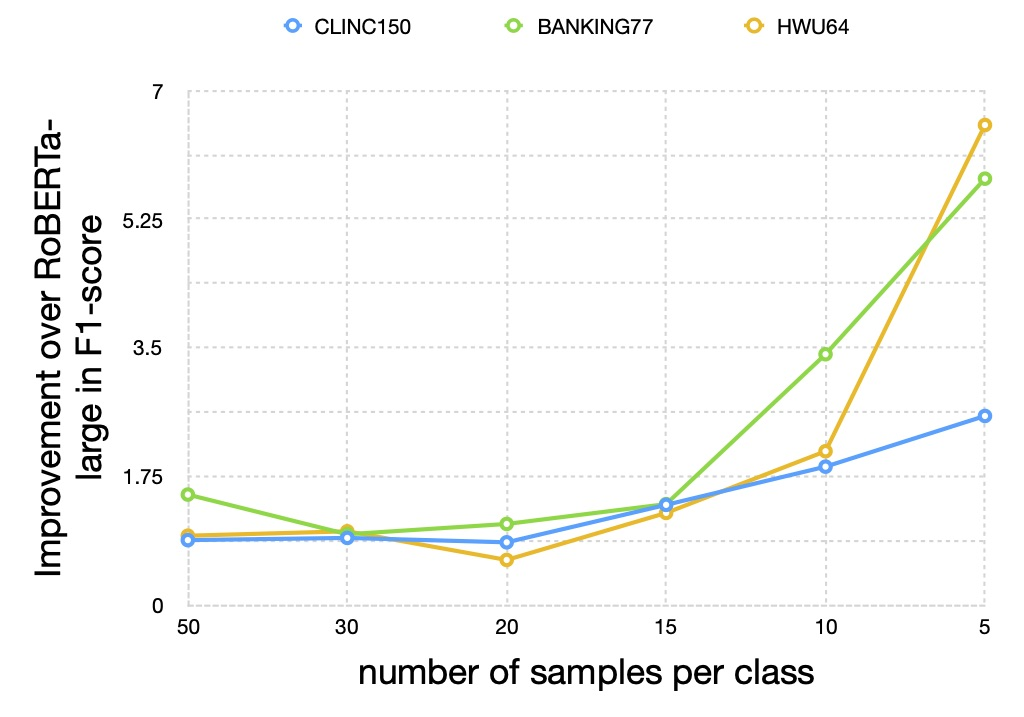
\includegraphics[scale=0.2]{picture/improvement_trend.jpg} 
      \par
    \end{centering}
    \caption{
      Improvements with different size of training data.
    }
    \label{fig:trend}
  \end{figure}

  Especially,  in the most extreme few-shot setting with only 5 training samples
  per  class  our joint SFC achieves 4.97 percent points improvements on average
  over  RoBERTa-large classification model . This observation indicates that SFC
  is  especially  well-performed  when being applied during the initial stage of
  building  task-specific  chatbot  system,  where the amount of data sample for
  each class label is extremely scarce.

  Furthermore,  our  proposed  joint  SFC can also achieve 2.04 percents average
  improvement  over  RoBERTa-large classification model on all the data settings
  including  the  ones  with  large  scale,  30  to  50  samples per class. This
  indicates that joint SFC can still steadily outperforms pretrained model based
  baseline even if the data size grows bigger. However, the improvement is still
  more prominent when the data is scarce, which makes SFC an excellent model for
  low-resource chatbot scenario.

  \subsubsection*{How does joint SFC relate to the label  embedding based  LEAM?}
  LEAM performs consistently better than TextCNN by a large margin in all
  datasets. TextCNN is practically efficiently in task-specific chat
  applications, and LEAM shows its power in modeling labeling information.

  LEAM  does not perform as well as SFCs, since the first intuitive reason is it
  does  not use pretrained model as encoding module; and another critical reason
  is  in  task-specific  chat applications, it is common to have many intentions
  that are close to some others with a minor difference, and it is hard and even
  impossible  to  name  each  intention  with  a short clear name. One candidate
  solution  is  setting  a most standard sample as the label of that class. When
  using  non-pretrained  models  base  LEAM,  this is applicable. Yet when using
  pretrained  model  based, as the all labels can be hundreds of thousands, then
  this  can not be accommodated in a poplar 32 G Tesla V100 GPU. Actually, joint
  SFC  can  be  kind  of  understood  as  a  generalization form of LEAM. In the
  scenario when there is no clear class label, the relationship between a sample
  and  a class label is implicitly encoded as that between a sample and another
  sample  from  the  same  class, and this turns into a sentence pair similarity
  model.

  \subsubsection*{Settings  of  hyperparameters} 
  Finally, we analyze the effect brought
  by  different  settings  of  hyperparameters,  see  Table \ref{tbe:table3}. 

  We  conduct  experiments on 5 different settings of hyperparameters, which are
  the  number of candidate class number $K$ and the number of sentence pairs $P$
  for  each  class,  on  ITG  and Amazon-670K datasets to find the most suitable
  setting  of  these  2 hyperparameters. We control the total number of sentence
  pairs  sampled for each user query into about the same level of amount(50-60).
  Through  analyzing the experimental results shown in Table \ref{tbe:table3}, we
  find  that the best setting of hyperparameters might be different for datasets
  of  different  data  size.  The  class label number of ITG and Amazon-670k are
  similar  in  our  experimental setting, which is around 250. However the total
  amount of data points of ITG is approximately 2 times larger than Amazon-670k.
  Therefore,  the  setting of $K=5$ and $P=10$ is good enough for ITG since most
  of  the  classes  contains  over 10 data points. However, for Amazon-670k, the
  amount  of  data  sample  for  each  class  is  scarce, thus, we may need more
  candidate  classes to sample enough effective sentence pairs for sentence-pair
  model  layer  of  SFC.  In this way, the setting of $K=10$ and $P=5$ becomes a
  good choice. However, in spite of the effect on evaluation performance brought
  by different settings of hyperparameters, joint SFC still steadily outperforms
  two-stage  SFC  by  0.41  percents  in  overall  average  F1 score  on  ITG and
  Amazon-670k datasets.

  In  conclusion, to the best of our knowledge, these experimental results place
  joint  SFC as the best performing model on 5 diverse experimental datasets for
  text   classification   task,   especially   when   it's   under  low-resource
  task-specific conversational chatbot scenario.

  \section{Conclusion}
  In  this  work, we successfully proposed SFC, a joint system of classification
  model  and  sentence-pair similarity model with multi-task learning, which can
  effectively  alleviate  the  limitation of classification model and similarity
  model   for  low-resource  text  classification  tasks.  Experimental  results
  illustrate that our proposed system can achieve great improvement on 5 diverse
  datasets for task-specific chatbot system over several competitive single-task
  baseline  models. Furthermore, we especially analyze the excellent performance
  of SFC when facing the challenge brought by few-shot scenarios, which is quite
  common in real-world application of chatbot system.

  \bibliographystyle{aaai21}
  \bibliography{refs}

\end{document}
